\hbadness=100000
\documentclass[12pt]{article}
\usepackage{hyperref}
\usepackage[left=1in, right=0.5in, top=1in, bottom=1in]{geometry}
\usepackage{tabto}
\usepackage{booktabs}
\usepackage[table]{xcolor}
\usepackage{tabularx}
\usepackage{makecell}
\usepackage{array}
\usepackage{float}
\usepackage{longtable}
\usepackage{amsmath}
\usepackage{amssymb}
\usepackage{lmodern}
\usepackage{graphicx}
\usepackage{multicol}
\usepackage{subcaption}

% TITLE PAGE DETAILS
\title{\bfseries An Empirical Analysis of Instability in Classification Models for Recidivism Risk Prediction Caused By Dataset and Stochastic Sources} % just review
\author{\bfseries 
 Nikka Angela E. Naputo\\
 CMSC 199.1 Research in Computer Science I\\
 Division of Natural Sciences and Mathematics\\
 University of the Philippines Tacloban College\\
 {\small nenaputo@up.edu.ph}
}
\date{\today}

% ----START THE DOCUMENT----
\begin{document}
\sloppy % Prevent text from extending to other columns

% ----DISPLAY TITLE----
\maketitle 
\newpage 

% ----DISPLAY TABLE OF CONTENTS----
\tableofcontents 
\newpage

% ----1. INTRODUCTION----
\section{Introduction} 
\tab Assessing recidivism risk among offenders is significant to helping identify what risk factors need to be addressed in order to prevent offender recidivism~\cite{bonta2007risk, duwe2017out}. Machine learning (ML) models have been developed specifically for recidivism risk prediction due to its scalability, efficiency, and complex pattern and relationship detection. Statistical ML-based tools such as COMPAS~\cite{northpointe2015practitioner} and MnSTARR~\cite{duwe2014development} have been developed to predict recidivism risk in defendants. To further improve predictive accuracy and capture complex, non-linear relationships in recidivism data, other modern ML approaches have been explored such as tree-based models, support vector machines, gradient-boosted trees, and neural networks~\cite{duwe2017out}.\\

These models are used increasingly in actual sentencing decisions, such as COMPAS, which has influenced the sentencing of court cases like Loomis v State in 2013~\cite{loomis2016} and the Samsa v State in 2014~\cite{samsa2014}. As a result, concerns regarding fairness in these models have emerged. In 2016, ProPublica published a report claiming their analysis on the racial fairness of COMPAS found it to be more likely to misclassify black defendants as higher risk and white defendants as lower risk~\cite{propublica2016analysis}. The report garnered criticism for its choice of evaluation metrics, particularly its focus on error rates without considering the differences in recidivism rates across the racial groups. By using alternative metrics such as predictive parity and AUC, the critics found similar levels of predictive performance between Black and White defendants, suggesting that different fairness definitions can lead to contrasting interpretations of bias~\cite{dieterich2016compas, corbett2017algorithmic, flores2016false}. Moreover, developing prediction models that try to address group bias can actually result in inconsistent predictions for the individual-level as offenders with the same attributes could be interpreted unfairly due to group membership~\cite{greene2022forks, corbett2017algorithmic}. \\

% ===== PLEASE REVIEW THIS CAUSE IT GETS REFERRED TO LATER ======
Predictive inconsistency is a less explored aspect within the rich literature of ML recidivism prediction risk as most studies either focus on measuring predictive performance~\cite{duwe2017out, travaini2022machine, tollenaar2013method} and fairness~\cite{tolan2019machine, dressel2018accuracy, ngo2018traditional}. Predictive inconsistency refers to the generation of varied risk scores generated for the same offender due to different, yet equally justifiable, technical choices made during model development~\cite{greene2022forks}. This variability is related to model instability, the formal term used in ML literature referring to multiple models of the same structure producing different predictions on the same individual. A model that is considered unstable undermines its reliability as its predictions cannot be fully trusted~\cite{riley2023stability}, and this becomes particularly critical in risk-sensitive situations where inconsistent predictions could lead to catastrophic outcomes such as harm to humans, major economic loss~\cite{zhang2024reliability}, or in the case of assessing recidivism risk, unfair legal consequences for the defendants~\cite{greene2022forks}. \\

Model instability can be caused by factors such as small perturbations in the training data or nondeterministic factors in the model's learning process~\cite{riley2023stability, lopez2022instability}, which this paper distinguishes into two types respectively: dataset instability and stochastic instability.\\

Though prior studies on recidivism risk prediction using ML often examined these models' performance and fairness, comparatively little attention has been given to exploring their instability as existing literature either does a broad conceptual analysis on the factors that cause predictive inconsistency~\cite{greene2022forks}, or study the instability of actuarial tools used in recidivism risk prediction~\cite{helmus2015stability}, not ML models. Moreover, as these models are being used in sentencing decisions, their predictions carry profound and potentially detrimental impact on an individual's legal status and personal freedom~\cite{van2022predicting}. \\

Therefore, examining the instability of ML models in recidivism risk prediction is essential, as it addresses significant concerns regarding a model's prediction reliability and the risk that inconsistent predictions could lead to, such as unfair legal outcomes and sentencing decisions, while filling a clear gap in the current literature.\\
\newpage

% ----1.1 BACKGROUND OF THE STUDY
\subsection{Background of the Study}
\subsubsection{Recidivism Risk Assessment} 
\tab Recidivism risk assessment is the use of statistical or algorithmic tools to predict the likelihood an individual will re-engage in criminal behavior after being punished or released~\cite{ozkan2017predicting}. These instruments serve as tools that help judges, administrators, and correctional officers make informed decisions regarding pretrial detention, sentencing, and inmate placement~\cite{corbett2017algorithmic}.\\

\textbf{There are four generations of risk assessment tools:}
\begin{enumerate}
 \item \textbf{First Generation (Pre-1950s):} Offender risk assessment was primarily based on subjective, professional judgements made by correctional staff~\cite{duwe2017out,ozkan2017predicting}. However, these assessments were often vulnerable to individual bias and inconsistency.
 \item \textbf{Second Generation (Late 1920s-1970s):} This era saw the introduction of objective actuarial methods which focused on static factors such as criminal history~\cite{duwe2017out}. 
 \item \textbf{Third Generation:} Recognizing the limitations of the second generation risk assessment tools, these tools began incorporating dynamic risk factors (criminogenic needs), which are factors that change over time and serve as targets for intervention, such as employment status or substance abuse, alongside static factors~\cite{duwe2017out}. 
 \item \textbf{Fourth Generation:} These are the modern recidivism risk assessment tools that continuously assess defendants throughout their involvement in the justice system, tracking changes over time and considering both risk and protective factors to guide the decisions of criminal justice practitioners~\cite{duwe2017out}.
\end{enumerate}

The evolution of these tools reflects a shift toward more data-driven and dynamic approaches to risk assessment, which has paved the way for the integration of ML techniques in recidivism risk prediction.

\subsubsection{Machine Learning}
\tab Machine Learning (ML) is a branch of artificial intelligence that focuses on algorithms capable of learning patterns from data without explicit programming~\cite{duwe2017out}. ML models are commonly categorized into two types based on their learning approach. Supervised learning models are trained using labeled data with known outcomes and are used to generate predictions. In contrast, unsupervised learning models are developed using unlabeled data and aim to identify patterns, structures, or relationships within the dataset~\cite{badillo2020introduction}.\\

Supervised learning has been applied across multiple domains such as healthcare, finance, marketing, engineering, and criminal justice due to its ability to model complex relationships and efficiently process large volumes of data~\cite{duwe2017out,ozkan2017predicting}. In the context of criminal justice, supervised ML models are used in risk assessment to support decision-making processes, such as prioritizing limited resources toward higher-risk defendants and informing interventions for those assessed as lower risk. 

\subsubsection{Machine Learning For Recidivism Risk Prediction}
\tab Since the 1990s, ML-based recidivism risk assessment tools have been developed to predict the likelihood of reoffending. Examples include the Correctional Offender Management Profiling for Alternative Sanctions (COMPAS), developed by Northpointe in 1998 using statistical and ML methods~\cite{northpointe2015practitioner}, and the Minnesota Screening Tool Assessing Recidivism Risk (MnSTARR), developed by Duwe in 2014 which utilizes multiple logistic regression modeling due to its interpretability that allows researchers to discern exactly how much each variable contributes to a final prediction~\cite{duwe2014development}.\\

These tools are used to support criminal justice decisions such as sentencing, pretrial detention, and offender supervision. In some cases, judicial decisions have been influenced by the outputs of these models. For example, in the case of Eric Loomis in 2013, the COMPAS assessment included in his Pre-Sentence Investigation (PSI) labeled him as “high risk” for recidivism, which was considered during sentencing~\cite{loomis2016}. Similarly, in the case of Jordan Samsa in 2014, the court considered components of the COMPAS report, such as criminogenic needs, in determining sentencing outcomes~\cite{samsa2014,liu2019beyond}.\\

Beyond existing risk assessment tools, general supervised ML models have also been explored for recidivism risk prediction such as logistic regression, random forests, gradient-boosted trees, and support vector machines~\cite{duwe2017out,ozkan2017predicting,ngo2018traditional}.

% EDIT THIS PART
\begin{enumerate}
 \item \textbf{Logistic Regression} \\
  \tab Logistic Regression (LR) is a statistical model used for binary classification tasks and is the most used baseline model in recidivism risk prediction studies due to its simplicity and interpretability~\cite{travaini2022machine}, which makes it particularly suitable for high-stakes domains such as criminal justice, where understanding model decisions is important. Moreover, it was used in the development of the MnSTARR~\cite{duwe2014development}.\\

  The way it works is by producing probability values between 0 and 1 for an outcome by inputting a linear combination of input features into a sigmoid function. \\
  
  The model estimates the probability of an event occurring using the equation \[ P(Y_i)=\frac{1}{1+e^{-(b_0+\sum_{j=1}^{p} b_j X_{ji})}} \] where the entire fraction represents the sigmoid (or logistic) function that maps any real-valued input into the ([0,1]) range. The term $ b_0 + b_1X_{1i} $ inside the exponent is the linear predictor, which combines the input feature $ X_{1i} $ with its corresponding coefficient $ b_1 $, along with the intercept $ b_0 $, The exponential constant $ e $ ensures a smooth, non-linear transformation of this linear predictor, allowing the model to produce probabilities rather than unbounded outputs.\\
  
  The predicted value $ P(Y_i) $ represents the probability that the outcome $ Y $ is true for a given instance $ i $, which can then be converted into a class label using a decision threshold (commonly 0.5).\\
  
  Each coefficient $ b_1 $ reflects the strength and direction of the relationship between the feature $ X $ and the log-odds of the outcome. This is what attributes LR's interpretability as each coefficient can be directly linked to changes in the predicted probability.\\

 \item \textbf{Random Forest}\\
  \tab Random Forest (RF) is an ensemble learning method that constructs multiple decision trees and combines their predictions to form a robust model~\cite{kovalchuk2023prediction}. It operates by generating a collection of decision trees trained on different bootstrap samples of the dataset and aggregating their outputs through a voting mechanism.\\
  
  Despite being less interpretable than simpler models like LR, RF is widely used in recidivism risk prediction due to its high accuracy, resistance to overfitting, and ability to handle high-dimensional data~\cite{kovalchuk2023prediction}, making it well-suited for real-world datasets, and thus why it is the second most popular model studied in the literature of recidivism risk prediction~\cite{travaini2022machine}.\\

  The prediction of the model can be expressed as \[\hat{y} = \text{mode}\{T_1(x), T_2(x), \dots, T_B(x)\} \] where each $ T_b(x) $ represents the prediction of the $b$-th decision tree and $B$ is the total number of trees in the forest. The function $\text{mode}(\cdot)$ corresponds to the majority voting scheme used in classification tasks, selecting the class most frequently predicted across all trees. Each individual tree is trained on a randomly sampled subset of the data (with replacement), a process known as bootstrap sampling, which introduces diversity among the trees. Additionally, at each split in a tree, only a random subset of features is considered, further reducing correlation between trees and improving generalization. The final prediction $\hat{y}$ is therefore more robust than that of a single decision tree, as it averages out errors and reduces variance. This ensemble approach allows RF to capture complex, nonlinear relationships in the data while mitigating the risk of overfitting.\\  

 \item \textbf{XGBoost}\\
  \tab XGBoost is a gradient-boosted tree algorithm that builds the model sequentially by correcting the errors of previous trees. It constructs an additive model where each new tree is trained to minimize the residual errors of the existing ensemble.\\
  
  Multiple studies have explored XGBoost in recidivism risk prediction, with results showing it yielded competitive or superior performance as compared to other models~\cite{won2019recidivism,rajendran2021predicting}. The model, combined with extensive feature engineering and hyperparameter tuning, was also used in the winning solution of the National Institute of Justice (NIJ) Recidivism Forecasting Challenge~\cite{han2022xgboost}. 
  
  The prediction of the model can be expressed as \[ \hat{y}_i = \sum_{t=1}^{T} f_t(x_i) \] where each $f_t(x_i)$ represents the prediction of the $ t$ -th decision tree and (T) is the total number of trees. Each function $ f_t $ belongs to the space of regression trees, and is added sequentially to improve the overall model performance. The training process minimizes an objective function defined as \[ \mathcal{L} = \sum_{i=1}^{n} l(y_i, \hat{y}_i) + \sum_{t=1}^{T} \Omega(f_t) \] where $ l(y_i, \hat{y}_i) $ is the loss function that measures the difference between the true value and the predicted value, and $ \Omega(f_t) $ is a regularization term that penalizes model complexity. This regularization component helps prevent overfitting by controlling the depth and structure of each tree.\\
  
  Unlike Random Forest, which builds trees independently, XGBoost builds trees sequentially, with each new tree focusing on correcting the errors made by previous ones. This boosting mechanism allows the model to capture complex patterns and improve predictive accuracy. The final prediction $ \hat{y}_i $ is therefore a weighted combination of all trees in the ensemble.\\
  
  Due to its optimization techniques, such as gradient-based learning and regularization, XGBoost is both computationally efficient and highly accurate. 

 \item \textbf{Linear Support Vector Machines (SVMs)}\\
  \tab Support vector machines are classification models that separate classes by finding a decision boundary that maximizes the margin between them. SVMs have been explored in recidivism risk prediction studies alongside other ML models, often demonstrating competitive performance across different evaluation settings~\cite{duwe2017out, tolan2019machine,ozkan2017predicting}. 
  
  There are two types of SVMs explored in recidivism risk prediction studies: linear (where classes can be linearly separated) and nonlinear SVMS (using of complex boundaries to separate classes)~\cite{tollenaar2013method, duwe2017out, dressel2018accuracy}. For this paper, only linear SVM will be discussed further.

  The decision function of a linear SVM can be expressed as \[ f(x_i) = w^T x_i + b \] where $ w $ is the weight vector, $ x_i $ is the feature vector for instance $i$, and $b$ is the bias term. This function defines a hyperplane that separates the classes in the feature space. The predicted class label is determined by the sign of the decision function, given by \[ \hat{y}_i = \text{sign}(w^T x_i + b) \] where positive and negative values correspond to different classes. The model is trained by solving an optimization problem that maximizes the margin while penalizing misclassifications, expressed as \[ \min_{w,b} \ \frac{1}{2} \|w\|^2 + C \sum_{i=1}^{n} \xi_i \] where $ \|w\|^2 $ controls the margin size, $ C $ is a regularization parameter, and $ \xi_i $ are slack variables that allow for some classification errors. This formulation ensures that the model balances margin maximization with classification accuracy. The resulting decision boundary is therefore the one that maximizes separation between classes while tolerating limited violations.
\end{enumerate}

\subsubsection{Concerns in Machine Learning-Based Risk Assessment}
\tab With the increasing use of ML models in criminal justice decision-making, several concerns have been raised regarding their application.\\

One major concern involves the fairness of these models. In 2016, ProPublica published an analysis of the COMPAS risk assessment tool, reporting that it was more likely to misclassify Black defendants as higher risk and White defendants as lower risk~\cite{propublica2016analysis}. The report garnered criticism from both Northpointe (the owner of COMPAS) and other researchers for its choice of evaluation metrics, particularly its focus on error rates without considering the differences in recidivism rates across the racial groups. By using alternative metrics such as predictive parity and AUC, the critics found similar levels of predictive performance between Black and White defendants, suggesting that different fairness definitions can lead to differing interpretations of bias~\cite{dieterich2016compas, corbett2017algorithmic, flores2016false}. Moreover, developing prediction models that optimize fairness such as group bias could result in inconsistent individual-level predictions as offenders with the same attributes could be interpreted differently due to group membership~\cite{greene2022forks, corbett2017algorithmic}.

Predictive inconsistency is a less extensively explored concern within the ML recidivism risk prediction literature as most studies focus on measuring predictive performance~\cite{duwe2017out, travaini2022machine, tollenaar2013method} and fairness~\cite{ tolan2019machine, dressel2018accuracy,ngo2018traditional} . Predictive inconsistency refers to the variability in risk scores assigned to the same individual due to different, yet equally justifiable, technical decisions made during model development~\cite{greene2022forks}. This variability is closely related to model instability, where models with the same structure may produce different predictions for the same individual~\cite{greene2022forks}.

\subsubsection{Instability in Machine Learning}
\tab Instability in ML refers to the sensitivity of a model's predictions to small changes in its training conditions~\cite{sun2015stability}. The most commonly discussed form of instability is dataset instability, which refers to the variability in a model's predictions due to small perturbations in the training data, such as resampling from the original dataset, removing individual data points, or introducing noisy data~\cite{riley2023stability,hardt2016train}. Another form of instability is stochastic instability, which arises from nondeterministic factors in the training process, such as random initialization and data ordering during learning~\cite{lopez2022instability}. This randomness, typically controlled through the model's random seed, can cause models to produce different predictions across runs.\\

An unstable model undermines reliability, as its predictions may not be consistent or dependable~\cite{riley2023stability}. This becomes particularly critical in risk-sensitive contexts, where inconsistent predictions may lead to harmful or high-cost outcomes~\cite{zhang2024reliability}. In the domain of criminal justice, the use of unstable models for recidivism risk assessment could result in unfair legal outcomes for defendants~\cite{greene2022forks}.

% ----2. RELATED WORKS----

\section{Related Works}
\tab A large volume of work in recidivism risk prediction focuses on evaluating the overall predictive performance of different ML approaches, particularly comparing traditional models with modern ones.\\

Duwe and Kim~\cite{duwe2017out} compared 12 supervised learning algorithms, including logistic regression, random forests, support vector machines, neural networks, and boosting techniques, using a large dataset of offenders released from prison. Their evaluation considered multiple dimensions of predictive validity, such as discrimination, calibration, and accuracy, across different scenarios varying in sample size, base rates, and predictor sets. While some ML methods, particularly boosting-based approaches like LogitBoost, achieved slightly higher predictive performance, the overall differences between models were relatively modest. This is similar to the findings of Travaini et al.~\cite{travaini2022machine}, who provided a comprehensive overview of the growing application of ML techniques in recidivism risk prediction. Their study analyzed multiple empirical works employing various datasets and models, including logistic regression, random forest, neural networks, and ensemble approaches, to evaluate predictive performance using metrics such as accuracy and AUC. Their findings indicate that across studies, most ML models achieve relatively strong predictive performance, with average results suggesting reliable classification of recidivism outcomes but that no single model consistently outperforms others.\\

These studies highlight that although more complex ML models are capable of capturing nonlinearities and high-dimensional interactions, their practical advantage in recidivism risk prediction is often limited, with simpler statistical models continuing to provide competitive performance. Moreover, model predictive performance is also context-dependent, meaning it is influenced by factors besides model structure.\\

Other than predictive performance, researchers have also increasingly examined the fairness and ethical implications of using ML models in criminal justice settings.\\

Tolan et al.~\cite{tolan2019machine} evaluated the predictive performance and fairness of ML models in comparison to structured human risk assessments within a juvenile justice context. Using a dataset of Catalonian youth offenders, they compared multiple ML models against the SAVRY framework, a structured professional judgement tool used by experts. Their results showed that ML models achieved slightly higher predictive performance, with AUC values improving when more features were included. However, this improvement came at the cost of fairness, as the models exhibited disparities across demographic groups, particularly with respect to sex and nationality. For instance, certain groups such as foreign nationals were more likely to be incorrectly classified as high risk, even when they did not recidivate. The study highlights a fundamental trade-off between predictive performance and fairness, demonstrating that optimizing for accuracy can introduce or amplify biases present in the data. This aligns with an earlier investigation by ProPublica~\cite{propublica2016analysis}, where they raised concerns regarding racial bias in COMPAS by conducting an empirical analysis of over 10,000 defendants from Broward County, Florida. Their study compared COMPAS risk predictions with actual recidivism outcomes over a two-year period and found that, while overall accuracy was moderate (around 61\%), the errors were distributed unevenly across racial groups. Specifically, Black defendants were significantly more likely to be falsely classified as high risk despite not reoffending, while White defendants were more likely to be incorrectly labeled as low risk despite recidivating. Even after controlling for factors such as prior offenses, age, and gender, Black defendants were still more likely to receive higher risk scores. These findings suggest that algorithmic predictions may systematically disadvantage certain demographic groups, raising critical concerns about fairness in risk assessment tools.\\ 

The ProPublica investigation ultimately sparked widespread debate on the ethical implications of using ML in criminal justice decision-making. Representing Northpointe, Dieterich et al.~\cite{dieterich2016compas} reanalyzed the same Broward County dataset and challenged the claim of racial bias. Their study argued that ProPublica relied on incorrect classification statistics, particularly focusing on false positive and false negative rates without accounting for differing base rates of recidivism across racial groups. By instead evaluating metrics such as predictive parity and AUC, they found that COMPAS exhibited similar predictive accuracy for Black and White defendants, indicating what they termed ``accuracy equity''. Their results showed that differences in error rates could arise naturally from underlying differences in group distributions, rather than from algorithmic bias. Consequently, they concluded that fairness assessments depend heavily on the choice of evaluation metric, and that alternative definitions can lead to different interpretations of bias. In addition, Flores et al.~\cite{flores2016false} provided a critical response to the ProPublica analysis, arguing that its conclusions were based on methodological and statistical shortcomings. They emphasized that ProPublica did not follow established standards for testing predictive bias and instead relied on inappropriate comparisons of group-level error rates. Using alternative analytical approaches, including AUC comparisons and regression-based methods, they found no consistent evidence of racial bias in the predictive performance of COMPAS. Their findings reinforce the argument that conclusions about bias are highly sensitive to the evaluation framework and statistical methodology employed.\\

Studies have also explored how adhering to fairness metrics could result in inconsistent predictions for individuals. One such study is explored by Corbette-Davies et al.~\cite{corbett2017algorithmic}, where they investigate the inherent mathematical and ethical trade-offs between maximizing safety and satisfying various formal definitions of algorithmic fairness. By reformulating fairness as a constrained optimization problem, the authors demonstrate that adhering to common fairness metrics, such as statistical parity, conditional statistical parity, and predictive equality (equal false positive rates), requires the application of different, race-specific risk thresholds wherein the threshold for  for white defendants are lowered while the threshold for black defendants are increased, while the development of a model focused on maximizing safety applies a single, uniform threshold to all individuals. Using the data from Broward County for their simulation, the authors found that the fair models led to the detainment of 17\% low-risk offenders and a 9\% increase in violent crime due to the release of higher-risk offenders. Moreover, individual outcomes (detention or release) are inconsistent as a black defendant with the exact same risk score as a white defendant could be released, with the latter being detained solely to satisfy the group-level fairness constraint. 

Predictive inconsistency is a less explored aspect within the ML recidivism risk prediction  literature despite multiple studies focusing on measuring predictive performance and fairness. Greene et al.~\cite{greene2022forks} defines predictive inconsistency as the phenomenon where equally justifiable modeling decisions can produce different predicted risk scores for the same individual. This perspective highlights that variability in predictions does not solely arise from model randomness, but also from technical choices made throughout the model pipeline, including data selection, preprocessing, and model structure. Similar to Corbette-Davies et al., Greene et al. mentions fairness selection as one of these "forking paths" as there is no single definition to fairness. In high-stakes domains such as criminal justice, such inconsistencies raise concerns regarding the reliability and legitimacy of algorithmic risk assessment tools.\\

The variability described by Greene et al. can be understood in relation to model instability, the formal term used within ML literature that refers to the variability of predictions that are caused by small perturbations in the training data or stochastic elements in the training process. This connects to algorithmic stability explored by Sun~\cite{sun2015stability} where it is defined as the consistency of a model's predictions under small perturbations in the training data. Through both theoretical analysis and empirical experiments, Sun demonstrated that models with similar predictive accuracy can exhibit significantly different levels of stability, highlighting that accuracy alone is insufficient to evaluate model behavior. The findings emphasize that unstable models may undermine reproducibility and user trust, especially in applications where consistent predictions are critical. \\

% dataset and stochastic instability
Model instability has been explored in other domains, such as in healthcare. Riley and Collins~\cite{riley2023stability} proposed a comprehensive framework for evaluating instability in clinical prediction models across multiple levels. Their approach uses bootstrap resampling to repeatedly reconstruct models from the same dataset, allowing the assessment of how predictions vary under small perturbations in the training data. The study defines several levels of instability, including variability in overall estimated risk, changes in the distribution of predictions, subgroup-level instability, and instability at the individual prediction level. To quantify these effects, they introduced measures such as the mean absolute prediction error (MAPE), which captures the deviation between predictions from bootstrap models and the original model. Their findings demonstrate that even small changes in the dataset can lead to noticeable variability in model predictions, particularly in small sample sizes or high-dimensional settings, despite stable overall performance metrics. This variability was especially evident at the individual level, where predictions for the same individual could differ significantly across models. These results highlight how small changes in the dataset can influence model instability in clinical settings, potentially affecting clinical decision-making, and emphasize the need to evaluate models beyond traditional performance metrics. \\

Beyond dataset-related sources of variability, instability can also arise from the stochastic nature of model training itself. Lopez-Martinez et al.~\cite{lopez2022instability} further examined instability in clinical risk prediction models, particularly focusing on deep learning approaches used for risk stratification. Using electronic health record (EHR) data, they conducted repeated training runs of identical models with different random seeds and showed that model predictions can vary significantly at the individual level despite similar aggregate performance metrics such as ROC-AUC and PR-AUC. To quantify this variability, they introduced metrics such as the Top-K Jaccard similarity, which measures the consistency of high-risk individuals selected across model runs, and rank correlation measures to assess stability in prediction ordering. Their results demonstrate that deep learning models tend to exhibit greater instability compared to simpler models such as logistic regression, particularly in scenarios involving resource allocation where only top-risk individuals are considered. Additionally, the study showed that instability can lead to inconsistent decision-making and variability in subgroup representation, raising concerns about fairness and reliability in deployment settings.\\

% model reliability
While stability focuses on variability in predictions, a closely related concern is the reliability of individual predictions. The importance of reliability in predictive systems has been highlighted by Zhang and Bose~\cite{zhang2024reliability}, who introduced the Model Reliability for Individual Prediction (MRIP), a quantitative framework that measures the reliability of a model's prediction at the individual level rather than relying on aggregate metrics. Specifically, MRIP evaluates the probability that a model's prediction remains within an acceptable error range under small perturbations of the input, thereby capturing local uncertainty and variability in predictions. Their findings emphasize that aggregate performance metrics such as MSE or accuracy are insufficient for high-stakes applications, as models with strong overall predictive performance may still produce large errors for specific individuals. Similarly, Biddle~\cite{biddle2022predicting} examined the epistemic risks inherent in ML systems, particularly in the context of recidivism risk prediction. Drawing from philosophy of science, the study argues that predictive models are inherently value-laden, as their design involves trade-offs between different types of errors and uncertainties that can disproportionately impact individuals. In high-stakes domains such as criminal justice, these epistemic risks translate into real-world consequences, where unreliable predictions may lead to unjust or harmful decisions. Together, these works highlight that beyond accuracy and fairness, understanding and quantifying the reliability of individual predictions is crucial for the responsible deployment of ML systems.\\

Despite the growing body of work focusing on predictive performance and fairness, there are still limited empirical studies on instability in ML-based recidivism risk prediction literature. One notable study by Helmus and Thornton~\cite{helmus2015stability} examined the stability of actuarial risk assessment tools by analyzing the predictive consistency of individual items across multiple samples. Their findings showed that while most items were generally predictive, roughly half exhibited variability in predictive accuracy across different populations, indicating that risk estimates are not entirely stable. This variability was often observed in the magnitude rather than the direction of prediction, suggesting that risk factors may behave differently depending on contextual and sample-specific conditions. However, this line of work focuses on traditional actuarial instruments such as Static-99R and Static-2002R, and does not extend to modern ML-based approaches.\\

Overall, the existing literature demonstrates that while substantial progress has been made in evaluating recidivism risk prediction models in terms of predictive performance and fairness, these perspectives alone are insufficient to fully understand model behavior. Studies on model instability highlight that models with similar aggregate performance can produce significantly different predictions at the individual level, influenced by factors such as data perturbations and stochastic training processes. Furthermore, research in other domains, particularly healthcare, shows that such instability is not merely theoretical but can have practical consequences for decision-making, reinforcing the importance of evaluating prediction variability. Despite these insights, the application of instability and reliability analysis to ML-based recidivism risk prediction remains limited, with existing work focusing on traditional actuarial tools. This gap motivates the present study, which aims to empirically analyze the instability of ML models in recidivism risk prediction, considering both dataset and stochastic sources of variability, and to assess how such instability affects individual-level predictions while also evaluating model predictive performance, fairness, and reliability.

% ----3. STATEMENT OF THE PROBLEM----

\section{Statement of the Problem} 
\tab ML models are increasingly used in recidivism risk prediction to support decision-making processes within the criminal justice system, particularly in assessing a defendant's risk of reoffending. While numerous studies have focused on evaluating the predictive performance and fairness of these models, comparatively limited attention has been given to their stability. Model instability, which refers to the variability of predictions under small changes in training data or stochastic processes, may result in different predictions for the same individual across model runs or different modeling conditions. This phenomenon is closely related to the broad concept of predictive inconsistency, where equally valid modeling choices can yield divergent outcomes. In high-stakes domains such as criminal justice, such inconsistencies raise concerns regarding the reliability and trustworthiness of algorithmic risk assessments, as they may influence decisions that affect a defendant's personal freedom and legal status.\\

Although prior research has explored instability in traditional actuarial risk assessment tools or conducted a conceptual analysis on the forking paths that cause predictive inconsistency, there remains a lack of empirical studies examining instability in ML-based recidivism risk prediction models. In particular, it is unclear to what extent these models exhibit instability when subjected to variations in training data and stochastic factors during training. Furthermore, the manner in which instability manifests across different evaluation dimensions, such as predicted scores, ranking of individuals, classification outcomes, contextualized with predictive performance, fairness, and reliability, remains underexplored. It is also not well understood how instability varies across different model types or which input features contribute most to unstable predictions.\\

This study addresses these gaps by empirically analyzing the instability of classification models used in recidivism risk prediction. Specifically, it examines how model predictions vary under perturbations in the training data and stochastic training conditions, evaluates instability alongside predictive performance, fairness, and reliability metrics, and identifies key factors that contribute to variability in predictions.

\section{Objectives of the Study} 
\subsection{General Objective} Evaluate the instability of classification models used in recidivism risk prediction through dataset and stochastic factors.
\subsection{Specific Objectives}
\begin{enumerate}
 \item Generate bootstrapped samples from the training dataset and retrain the models to assess dataset instability.
 \item Retrain models on the same dataset with different random seeds to assess stochastic instability.
 \item Evaluate each model for each type of instability using metrics for instability, performance, fairness, reliability, and feature contributions using the prediction values obtained. 
 \item Analyze how results obtained from metrics evaluating each type of instability and model structure influences overall model instability. 
\end{enumerate}

\section{Significance of the Study}
\tab This study contributes to the growing body of research on ML recidivism risk prediction by addressing a relatively underexplored aspect: model instability. While prior studies have largely focused on evaluating model predictive performance and fairness, this research focuses on model instability, which is closely related to both predictive inconsistency and reliability. Studying it highly significant within a high\-stakes domain such as criminal justice where model outputs may influence legal decisions and defendant outcomes.\\

By empirically analyzing both dataset instability and stochastic instability across multiple classification models, this study provides a deeper understanding of how and why prediction variability occurs. The findings offer insights into the extent to which different models produce inconsistent predictions for the same defendant, highlighting potential risks in their deployment. This contributes to more informed model selection and evaluation practices beyond traditional performance metrics.\\

Furthermore, the integration of instability, performance, and reliability metrics, including individual-level reliability assessment, advances current evaluation frameworks by demonstrating that high predictive accuracy does not necessarily imply consistent or trustworthy predictions. This is particularly valuable for researchers and practitioners seeking to develop more robust and dependable ML systems for recidivism risk prediction.\\

The study also benefits policymakers and stakeholders in the criminal justice system as it raises awareness of the potential consequences of relying on unstable predictive models. By identifying factors that contribute to instability, including feature-level variability through SHAP analysis, the research supports the development of decision-support tools that account for the features influencing model predictions.\\

Ultimately, this study fills a critical gap in the literature by linking instability with predictive performance, fairness, and reliability in recidivism risk prediction models, promoting a more thorough approach to evaluating ML systems in high-risk applications.

\section{Scope and Limitations} 
\tab This study focuses on two forms of empirical evaluation of model instability through controlled perturbations of the training data and stochastic initialization via random seed. The analysis measures predictive performance, fairness, reliability, and instability across multiple dimensions such as predicted scores, ranking of individuals, and classification outcomes.\\

The study is limited to classification models, as these provide a controlled and interpretable setting for analyzing prediction variability. More complex models, such as multi-class or deep learning architectures, are excluded to maintain clarity and consistency in the analysis. The models considered include logistic regression, random forests, support vector machines, and boosting-based approaches.\\

The dataset used in this study is limited to the COMPAS recidivism dataset, specifically the version in HuggingFace, due to its availability, preprocessing suitability, and sufficient sample size for repeated experimentation. As a result, the findings may not generalize to other datasets or domains with different characteristics.\\

This study assumes that the dataset is properly preprocessed by iModels and that model configurations are correctly implemented. It does not account for external factors such as data quality issues, feature engineering variations, or real-world deployment conditions. Additionally, while multiple instability metrics are used, they capture different aspects of variability and do not constitute a single unified measure of model instability.

\section{Proposed Methodology}
\tab This study aims to evaluate the instability of models used in ML recidivism risk prediction while contextualizing it through an analysis of its predictive performance, fairness, reliability, and feature contributions. The methodology will be conducted under two experimental regimes: (1) dataset instability experiments, where the model stochasticity is controlled through a fixed random seed $s = 0 $ to isolate the effect of data perturbations, and (2) stochastic instability experiments, where the dataset is held constant while model-internal randomness is varied through repeated runs using different random seeds  $ s = 1 ... 10 $. \\

The methodology is designed to ensure clarity, reproducibility, and controlled experimentation, allowing any variability in model outputs to be attributed specifically to either data perturbations or stochastic training processes. \\

The study does not intend to minimize dataset or stochastic instability, nor does it seek to optimize predictive performance, fairness, and reliability. It is instead focused on evaluating and explaining how prediction variability occurs under controlled perturbations. \\

The section consists of subsections regarding the dataset, model selection and configurations, evaluation metrics, tools, and experiment implementation.

\subsection{Dataset} 
\tab The dataset to be used will be a version of the ProPublica COMPAS Recidivism Dataset that has been one-hot encoded and split into training and testing sets by iModels, with 4.94k and 1.24k rows, respectively. The dataset is accessible on the HuggingFace website and can be directly imported into Python.\\

The following table describes each feature within the dataset:
\begin{longtable}{
 |>{\raggedright\arraybackslash}p{5cm}
 |>{\raggedright\arraybackslash}p{2cm}
 |>{\raggedright\arraybackslash}p{9cm}|
}
\caption{ProPublica COMPAS Recidivism Dataset on HuggingFace (One-Hot Encoded By iModels)}\\ \hline
\textbf{Column Name} & \textbf{Type} & \textbf{Description}\\ \hline
\endhead

age & INTEGER & Age of the defendant\\ \hline
priors\_count & INTEGER & No. of prior charges or criminal cases recorded for a defendant prior to the current offense \\ \hline
days\_b\_screening\_arrest & INTEGER & No. of days between the defendant's arrest and when they were screened by COMPAS \\ \hline
c\_jail\_time & INTEGER & No. of days a defendant was kept in jail for the entire duration of their charge \\ \hline
juv\_fel\_count & INTEGER & No. of prior juvenile felony charges \\ \hline
juv\_other\_count & INTEGER & No. of prior juvenile misdemeanor charges \\ \hline
juv\_misd\_count & INTEGER & No. of other prior juvenile charges \\ \hline
c\_charge\_degree\:F & BINARY & 1 if the current charge is a felony, 0 otherwise \\ \hline
c\_charge\_degree\:M & BINARY & 1 if the current charge is a misdemeanor, 0 otherwise\\ \hline
race\:African-American & BINARY & 1 if the race of the defendant is African-American, 0 otherwise \\ \hline
race\:Asian & BINARY & 1 if the race of the defendant is Asian, 0 otherwise \\ \hline
race\:Caucasian & BINARY & 1 if the race of the defendant is Caucasian, 0 otherwise \\ \hline
race\:Hispanic & BINARY & 1 if the race of the defendant is Hispanic, 0 otherwise \\ \hline
race\:Native\_American & BINARY & 1 if the race of the defendant is Native\_American, 0 otherwise \\ \hline
race\:Other & BINARY & 1 if the race of the defendant is Other, 0 otherwise \\ \hline
age\_cat\_\:25\_-\_45 & BINARY & 1 if the defendant is between 25 to 45 years old, 0 otherwise \\ \hline
age\_cat\_\:Greater\_than\_45 & BINARY & 1 if the defendant is greater than 45 years old, 0 otherwise \\ \hline
age\_cat\_\:Less\_than\_25 & BINARY & 1 if the defendant is less than 25 years old, 0 otherwise \\ \hline
sex\:Female & BINARY & 1 if the defendant is a woman, 0 otherwise \\ \hline
sex\:Male & BINARY & 1 if the defendant is a man, 0 otherwise \\ \hline
is\_recid & BINARY & 1 if the defendant actually recidivated after the last COMPAS assessment, 0 if they did not \\ \hline
\end{longtable}

%ADD HERE THE DEFINITIONS OF THE MODELS TO BE USED

\subsection{Machine Learning Models and Configurations}
\tab The ML models to be used for training and evaluation are based on the following model types: statistical, tree-based, gradient-boosted tree, and support vector machine. The selection of a model for each of these are based on how frequently they are explored or cited in recidivism risk prediction literature. 

\begin{enumerate}
 \item \textbf{Statistical Model: Logistic Regression} \\
  \tab Logistic Regression (LR) is selected as the statistical model as it is the most explored model in ML recidivism risk prediction literature~\cite{travaini2022machine} and will serve as the baseline model. It is fitting for binary classification tasks, and is both simple to implement and highly interpretable. 

 \item \textbf{Tree-Based Model: Random Forest}\\
  \tab Random Forest (RF) is chosen as the tree-based model because it is it is the second most popular model studied in the literature of recidivism risk prediction~\cite{travaini2022machine}. The model has a high accuracy, is resistant to overfitting, and has the ability to handle high-dimensional data~\cite{kovalchuk2023prediction}.

 \item \textbf{Gradient-Boosted Tree: XGBoost}\\
  \tab XGBoost is selected as the gradient-boosted tree algorithm due to the model being explored in existing recidivism risk prediction literature~\cite{won2019recidivism,rajendran2021predicting}, where it shows competitive or superior predictive performance as compared to the other models. The model was also used in the winning solution of the National Institute of Justice (NIJ) Recidivism Forecasting Challenge~\cite{han2022xgboost}. Unlike the other models, XGBoost requires explicit parameter specification due to the absence of universally effective default settings. Hence, for this study, a set of predefined hyperparameters will be used to ensure stable and efficient training. 

 \item \textbf{Support Vector Machine: LinearSVC}\\
  \tab Though SVMs have been explored in recidivism risk prediction studies alongside other ML models, often demonstrating competitive performance across different evaluation settings, these papers often do not explicitly state the type of SVM used~\cite{duwe2017out, tolan2019machine,ozkan2017predicting}. For this study, a linear SVM will be used rather than a nonlinear variant due to its lower model complexity and interpretability. A linear decision boundary allows for a clearer analysis of how input features influence predictions, which is significant for an instability analysis. 
  
  The specific implementation to be used is LinearSVC, which is available in scikit-learn. It is computationally efficient, making it suitable for the study as the experiment will require multiple model retrainings.

  Unlike probabilistic models, LinearSVC does not inherently produce probability estimates, but instead outputs distance-based scores from the decision boundary. These scores can be transformed into probability estimates through post-hoc calibration methods such as Platt scaling or isotonic regression, which can be implemented using \texttt{CalibratedClassifierCV} in Python. This will allow the model to produce probability scores required for evaluation metrics.
\end{enumerate}

With regards to the inherent stochasticity of ensemble models such as Random Forest and XGBoost, care will be taken to distinguish dataset-induced instability. In particular, Random Forest introduces randomness through bootstrap sampling of the training data and random feature selection at each split, which can lead to variability in model outputs even under identical training conditions. For XGBoost, stochastic components such as subsampling and column sampling are likewise controlled or explicitly held constant when not part of the experimental design. This ensures that any measured variation in predictions reflects differences in data sampling rather than uncontrolled randomness within the learning algorithms themselves. \\

Each model will be implemented using the following controlled baseline configurations which are fixed across all experiments for both instability types while avoiding extensive tuning to ensure that no additional uncontrolled source of instability is introduced and that the experiment is reproducible across all experimental runs.

\begin{multicols}{2}
 \subsubsection*{1. Logistic Regression}
 \begin{itemize}
  \item penalty = L2
  \item solver = lbfgs
  \item max\_iter = 1000
  \item C = 1.0
  \item random\_state = $s$
 \end{itemize}

 \columnbreak

 \subsubsection*{2. Random Forest}
 \begin{itemize}
  \item n\_estimators = 100
  \item max\_depth = None
  \item bootstrap = True
  \item max\_features = sqrt
  \item random\_state = $s$
 \end{itemize}
\end{multicols}

\begin{multicols}{2}
 \subsubsection*{3. XGBoost}
 \begin{itemize}
  \item objective = binary:logistic
  \item max\_depth = 3
  \item learning\_rate = 0.1
  \item n\_estimators = 100
  \item subsample = 0.8
  \item colsample\_bytree = 0.8
  \item random\_state = $s$
 \end{itemize}

 \columnbreak

 \subsubsection*{4. LinearSVC}
 \begin{itemize}
  \item C = 1.0
  \item loss = squared\_hinge
  \item max\_iter = 1000
  \item random\_state = $s$
 \end{itemize}

 To obtain probability estimates, the model will be wrapped using:
 \begin{itemize}
  \item CalibratedClassifierCV
  \begin{itemize}
    \item method = sigmoid
    \item cv = 5
  \end{itemize}
 \end{itemize}
\end{multicols}

\subsection{Metrics for Instability}
To evaluate dataset and stochastic instability in each model, multiple instability metrics will be used to measure different aspects of variability such as score distributions, labels, and ranking. Other metrics will also be used to measure different aspects of each model such as performance, fairness, reliability, and feature contribution. Each instability type will be measured separately using the metrics.\\

Before presenting the metric formulations, the following notation will be used throughout the equations. Let: 
\begin{itemize}
  \item $ R $ denote the total number of model runs.
  \item $ D $ denote the total number of defendants in the dataset.
  \item $ K $ represent the size of the top-$K$ subset of defendants identified as highest risk.
\end{itemize}
\tab These variables will be used consistently across all defined metrics.

\begin{itemize}
  \item \textbf{Score Distribution-Level Instability: 95\% Stability Interval (SI)}\\
    \tab This will visualize the range of which predicted scores for each defendants are expected to fall across repeated runs~\cite{riley2023stability}. Wider intervals will indicate greater instability in the scores. The range of the interval is described through the following formula: \\
    \[
    \text{SI}_{95\%,d} =
    \left[
    Q_{0.025}\big(\{\hat{p}_d^{(r)}\}_{r=1}^{R}\big),
    \;
    Q_{0.975}\big(\{\hat{p}_d^{(r)}\}_{r=1}^{R}\big)
    \right]
    \] 
    where $ Q_{0.025} $ and $ Q_{0.975} $ denote the 2.5th and 97.5th percentiles of the predicted scores $ \hat{p}_d^{(r)} $ across all runs $ r = 1, \dots, R $.

  \item \textbf{Score-Level Instability: Mean Absolute Prediction Error (MAPE)}\\
    \tab This metric is used to quantify the average absolute difference in predicted scores for each defendant across runs~\cite{riley2023stability}. Higher MAPE values for a model will indicate greater variability in predicted risk scores, suggesting higher instability.\\

    Each MAPE value per defendant $ d $ is calculated using the formula:
    \[ \text{MAPE}_d=\frac{1}{R}\sum_{r=1}^{R}|\hat{p}_{d}^{(r)}-\bar{p}_d| \]
    where $ \hat{p}_d^{(r)} $ is the predicted probability for  defendant $ d $ in run $ r $ , $ \bar{p}_d $ is the mean predicted probability for  defendant $ d $ across all runs. \\

    To get the average MAPE for a model, we use the formula:
    \[ \overline{\text{MAPE}}=\frac{1}{D}\sum_{d=1}^{D}\text{MAPE}_d \]

  \item \textbf{Label-Level Instability: Classification Instability Index (CII)}\\ 
    \tab This metric is used to capture how often a defendant's predicted class label changes across repeated model runs. It measures the frequency with which a defendant's predicted classification (e.g., high-risk vs low-risk) changes across runs~\cite{riley2023stability}. Higher CII values will indicate greater instability in classification outcomes.\\

    The following formula is used to calculate the CII per defendant $ d $:
    \[ \text{CII}_d = \frac{\text{flips}_d}{\binom{R}{2}} \]

    where the no. of label flips per defendant $ \text{flips}_d $ is calculated using:
    \[ \text{flips}_d = \sum_{r<s} \mathbf{1}\big(y_d^{(r)} \ne y_d^{(s)}\big) \]
    
    $ y_d^{(r)} $ is the predicted class label for defendant $ d $ in run $ r $ , $ \mathbf{1}(\cdot) $ is the indicator function that equals 1 when the condition is true and 0 otherwise. \\

    Moreover, the total number of unique runs $ \binom{R}{2} $ is calculated using:
    \[ \binom{R}{2} = \frac{R(R-1)}{2} \] 

  \item \textbf{Ranking-Level Instability: Top-$ K$ Jaccard Similarity} \\
    \tab Evaluates whether the same defendants are consistently identified as high-risk across different model runs. It measures the overlap between the sets of defendants identified as highest risk (e.g., top 10\%) across different runs~\cite{lopez2022instability}. A lower Jaccard similarity will indicate greater inconsistency in identifying high-risk defendants.\\

    In this study, $K$ is defined as the top 10\% of defendants with the highest predicted risk scores. This threshold is fixed across all models and experiments to ensure consistent comparison of ranking instability.\\

    To get the Top-K Jaccard for a model, the following formula is used:
    \[ j(X_r^K,X_s^K)=\frac{|X_r^K \cap X_s^K|}{|X_r^K \cup X_s^K|} \]

    wherein the Jaccard of each top-K pair is calculated using the formula:
    \[ J=\frac{1}{\binom{R}{2}}\sum_{r<s}j(X_r^K,X_s^K) \]

    $ X_r^K $ and $ X_s^K $ represent the sets of top-$ K$ highest-risk defendants identified in runs $ r $ and $ s $ , respectively, and $ J $ is the average Jaccard similarity computed across all pairs of runs $ (r,s) $ such that $ r < s $ .
\end{itemize}

In addition to instability metrics, the models will be evaluated based on their predictive performance, as stability alone is insufficient without acceptable model performance. The following metrics will be used to measure the model's performance: \\

\textbf{Performance:} 
\begin{itemize}
  \item \textbf{Brier Score (BS)}\\
    \tab This will assess the accuracy of predicted scores~\cite{rufibach2010use}. The standard deviation of Brier scores across runs will also be computed to evaluate instability in probability accuracy. Higher variability will suggest inconsistency in the quality of probabilistic predictions, including potential variation in calibration.\\

    To get the Brier Score per run $ r=1, \dots, R $, the following formula will be used:
    \[ \text{BS}_r = \frac{1}{D} \sum_{d=1}^{D} \left( \hat{p}_d^{(r)} - y_d \right)^2 \]

    The average Brier Score per model is calculated using the formula:
    \[ \overline{\text{BS}}=\frac{1}{R}\sum_{r=1}^{R}\text{BS}_r \]

    and the standard deviation of a model's Brier Scores is computed using:
    \[ SD(\text{BS}) = \sqrt{ \frac{1}{R - 1} \sum_{r=1}^{R} \left( \text{BS}_r - \overline{\text{BS}} \right)^2 } \]

    where $ \hat{p}_d^{(r)} $ is the predicted probability for defendant $ d $ in run $ r $ , $ y_d \in \{0,1\} $ is the true outcome.

  \item \textbf{Calibration Plot}\\
  \tab This visualization assesses how well predicted scores align with observed outcome frequencies. A curve close to the diagonal indicates good calibration, while deviations suggest overconfidence or underconfidence in predictions.
  
  \item \textbf{ROC-AUC}\\
  \tab This metric evaluates the model's ability to distinguish between positive and negative classes across all classification thresholds. Higher ROC-AUC values indicate better discriminative performance.\\

  The following formulas calculate for the True Positive Rate and False Positive Rate for a model across thresholds $ t $:
  \[ \text{TPR}(t) = \frac{TP_t}{TP_t + FN_t} \]
  \[ \text{FPR}(t) = \frac{FP_t}{FP_t + TN_t} \]

  To calculate for the ROC-AUC per run $r$ of a model, we use the formula:
  \[ \text{ROC-AUC}_r = \sum_{t=1}^{T} (\text{FPR}_t - \text{FPR}_{t-1}) \cdot \text{TPR}_t \]
  which uses a discrete approximation of the area under the ROC curve across thresholds.

  \item \textbf{Performance-Level Instability: Standard Deviation of ROC-AUC} \\
  \tab This metric measures variability in ROC-AUC across repeated runs. Higher standard deviation indicates greater instability in model performance.

  \[ SD(\text{ROC-AUC})=\sqrt{\frac{1}{R-1}\sum_{r=1}^{R}(\text{ROC-AUC}_r-\overline{\text{ROC-AUC}})^2} \]
\end{itemize}

However, aggregated performance metrics alone do not reflect the reliability of  defendant predictions, which is critical in risk-sensitive applications. Thus, this study will also incorporate a fairness metric to contextualize the results with regards to racial groups, a reliability metric to assess the consistency and trustworthiness of model outputs, and a feature contribution metric to identify the main features that contribute to model instability. 

\begin{itemize}
  \item \textbf{Fairness: False Positive Rate (FPR) Difference Across Demographic Groups}\\
  \tab This metric evaluates whether the model produces different false positive rates across demographic groups, which provides contextual insight into how instability may disproportionately affect certain populations in recidivism risk prediction. In high-stakes settings such as criminal justice, a high false positive rate indicates that individuals who did not actually recidivate are incorrectly classified as high-risk. Differences in false positive rates across groups may suggest unequal treatment in model predictions.

  The False Positive Rate for a demographic group $g$ is calculated using the following formula:
  \[
  FPR_g = \frac{FP_g}{FP_g + TN_g}
  \]

  where $FP_g$ represents the number of false positives for group $g$, and $TN_g$ represents the number of true negatives for group $g$.

  To measure disparity between two demographic groups $g_1$ and $g_2$, the False Positive Rate Difference is computed as:
  \[
  \Delta FPR = |FPR_{g_1} - FPR_{g_2}|
  \]

  Higher $\Delta FPR$ values indicate greater disparity in false positive outcomes between demographic groups, while values closer to zero indicate more similar false positive rates across groups.

  For this study, the metric will primarily be evaluated across racial groups within the COMPAS dataset to provide contextual interpretation of the practical implications of model instability. The fairness metric is included as a supplementary contextual measure and is not intended to serve as the primary focus of the study.

  \item \textbf{Reliability: Model Reliability for Individual Prediction (MRIP)}\\ 
  \tab Quantifies the likelihood that a model's prediction error remains within an acceptable range for a given input~\cite{zhang2024reliability}, which measures the deviation between the true binary outcome and the predicted probability. This approach will provide a more granular measure of prediction reliability compared to traditional aggregate metrics and will be especially relevant in high-stakes decision-making contexts.
  \[
  \mathcal{R}(x_d) =
  P\left(
    \left| y_d^* - \hat{p}(x_d^*) \right| \le \epsilon
    \;\middle|\;
    x_d^* \in B(x_d)
  \right) \]
  \[ B(x_d) = \left\{ x_d^* \mid \| x_d^* - x_d \| \le \delta \right\} \]

  To operationalize MRIP, the following parameters will be defined:
  \begin{itemize}
    \item $\epsilon = 0.1$, representing the acceptable prediction error tolerance
    \item $\delta = 0.05$, representing the maximum perturbation radius
  \end{itemize}

  Perturbations $x_d^*$ will be generated by adding Gaussian noise to the input features: \[ x_d^* = x_d + \mathcal{N}(0, \sigma^2) \] 
  where $\sigma = 0.05 \cdot \text{std}(x)$, and values are clipped to remain within valid feature ranges.\\

  For each instance $x_d$, 50 perturbed samples will be generated, and MRIP will be estimated as the proportion of perturbed samples for which the prediction error satisfies: \[ |y_d - \hat{p}(x_d^*)| \le \epsilon \] where $ x_d $ is the original input for  defendant $ d $ , $ x_d^* $ is a perturbed version within the neighborhood $ B(x_d) $ , $ y_d^* \in \{0,1\} $ is the corresponding true outcome, $ \hat{p}(x_d^*) $ is the predicted probability, $ \epsilon $ is the acceptable error tolerance, and $ \delta $ controls the size of the neighborhood.

  \item \textbf{Feature Contribution: SHAP Analysis} \\
  \tab This method is used to further understand the sources of instability by identifying the features whose contributions to predictions vary most across runs~\cite{ponce2024practical}.\\

  The formula for SHAP analysis is:
  \[ f(x) = \mathbb{E}[f(x)] + \sum_{j=1}^{J} \phi_j(x) \]

  where $ \mathbb{E}[f(x)] $ is the expected model output over the dataset, and $ \phi_j(x) $ represents the contribution of feature $ j $ to the prediction for input $ x $ .
\end{itemize}

\subsection{Tools} 
All experiments will be conducted on the following device specifications:

\begin{table}[h]
  \centering
  \caption{Laptop Specifications Used in the Study}
  \begin{tabular}{|l|l|}
    \hline
    \textbf{Component} & \textbf{Specification} \\ \hline
    Model & Acer Aspire A315-44P \\ \hline
    Operating System & Linux Mint 22.3 (Ubuntu 24.04 base) \\ \hline
    Kernel & 6.17.0-19-generic (64-bit) \\ \hline
    Processor (CPU) & AMD Ryzen 7 5700U (8 cores, 16 threads) \\ \hline
    Graphics (GPU) & Integrated AMD Radeon Graphics \\ \hline
    Memory (RAM) & 16 GB \\ \hline
    Storage & 512 GB NVMe SSD (Samsung) \\ \hline
    Display & 1920 $\times$ 1080 @ 60Hz \\ \hline
    Desktop Environment & Cinnamon 6.6.7 \\ \hline
  \end{tabular}
  \label{tab:laptop_specs}
\end{table}

Moreover, the study will use the programming language Python for the development of the program due to its simple syntax, and rich ecosystem of libraries and frameworks, many of which are designed for ML development. The following Python libraries will be used: \\

\textbf{\texttt{datasets:}} Datasets provides one-line methods for importing any of the over nine hundred thousand public datasets available on the HuggingFace Datasets Hub. This library will be used to import the imodel's one-hot encoded version of the ProPublica COMPAS Recidivism Dataset.\\

\textbf{\texttt{pandas:}} Pandas provides data structure and data analysis tools that are easy to use, efficient, and high performing. The primary data structure to be used in the program will be the \texttt{DataFrame}, a two-dimensional table-like data structure consisting of rows and columns. This will be used for importing the training and test datasets, as well as storing and handling prediction outputs from csv files.\\

\textbf{\texttt{numpy:}} Numpy provides high-performance multidimensional arrays and tools used for efficient array operations. This will be used in the study for array-based computations, including operations involving the evaluation of instability in the models.\\

\textbf{\texttt{scikit-learn:}} Scikit-learn is an open-source library built for ML. It provides tools for data preprocessing, model training, and data analysis. This will serve as the primary library for implementing the models such as Logistic Regression, Random Forest, and LinearSVC, as well as evaluation metrics such as accuracy, precision recall curve, and brier score loss.\\

\textbf{\texttt{xgboost:}} The XGBoost Python library was built for high-efficiency implementation of gradient boosting. Because scikit-learn does not provide the XGBoost model and its methods, the study will source it from the xgboost library.\\

\textbf{\texttt{matplotlib:}} Matplotlib is a visualization library that is used to generate graphs and plots. In this study, it will be used to visualize each model's behavior such as their 95\% Instability Percentile and Classification Instability Distribution.\\

\textbf{\texttt{shap:}} The SHAP library provides tools for model interpretability through Shapley values. This will be used for implementing SHAP analysis on each of the prediction outcomes for dataset and stochastic instability to identify which features contribute most to instability and have the most variability in their SHAP values.\\

\subsection{Implementation}
\tab Figure 1 presents the flow of the proposed methodology for analyzing the instability within ML models used in recidivism risk prediction. 

\begin{figure}[h]
\centering
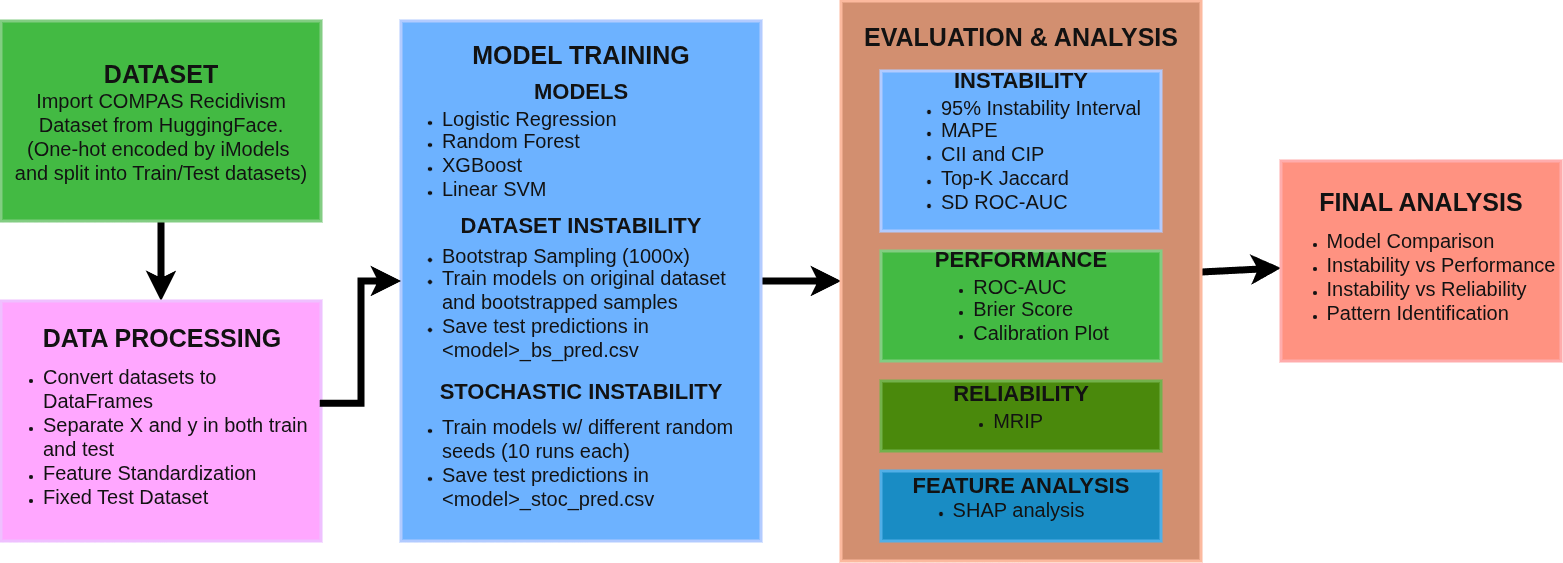
\includegraphics[width=1\textwidth]{proposed_methodology.png}
\caption{Overview of the proposed methodology for evaluating dataset and stochastic instability in ML models.}
\label{fig:Proposed Methodology Implementation}
\end{figure}

\begin{enumerate}
  \item \textbf{Dataset Importing and Processing:}
  The dataset is imported using the \texttt{datasets} library from HuggingFace. Since the source already contains separate training and test datasets, the program will import each dataset into panda DataFrames where the test dataset is fixed throughout all experiments and the training dataset is used for repeated model training.\\

  Because the selected version of the COMPAS Recidivism Dataset has already been one-hot encoded and prepared for ML use, only minimal preprocessing is required, specifically Feature standardization using \texttt{StandardScaler}. The scaler will be fit on the training data and subsequently applied to the test data using the same parameters to prevent data leakage. This preprocessing step is performed prior to model training and remains fixed across all bootstrap and stochastic iterations.\\

  Before performing repeated training procedures, each model will be trained once on the original training dataset using a fixed random seed $s = 0$. The predictions generated from this baseline model will serve as a reference for evaluating instability metrics.

  \item \textbf{Model Training For Dataset Instability:}
  To evaluate dataset instability, the study will employ bootstrap resampling approach~\cite{efron2000bootstrap}, which is a sampling method that generates proxy datasets by repeatedly drawing samples with replacement from the original dataset. This allows the study to simulate how model predictions may change under different possible versions of the same dataset. Moreover, bootstrapped resampling was also used by Riley and Collins~\cite{riley2023stability} in their study. The same hyperparameters will be held constant across all bootstrap iterations. \\

  A total of 1000 bootstrap samples will be generated from the original training dataset using sampling with replacement. This number is selected to ensure a stable estimation of prediction variability across runs while maintaining computational feasibility. Each bootstrapped dataset will maintain the same size as the original training set but will contain slight variations in data composition due to the resampling process. These variations will simulate realistic perturbations in the data, such as missing or duplicated observations. To ensure that dataset sources of instability are isolated from the stochastic sources, a fixed random seed $ s = 0 $ will be implemented for all dataset instability experiments.\\ 

  Each model will then be retrained independently on every bootstrapped sample with a fixed random seed of $ s = 0$. After training, predictions will be generated using the fixed test dataset and stored in structured CSV files with the filename $<model>\_bs\_pred.csv$, where each column represents the predicted scores from a specific training run. This organized storage will enable direct comparison of predictions across multiple runs for each individual.\\

  By repeating this process across all bootstrapped samples, the study will produce a distribution of predictions for each test instance which will serve as the basis for computing instability metrics in later stages of the methodology.

  \item \textbf{Model Training For Stochastic Instability:}
  To evaluate stochastic instability, models will be trained multiple times with different random seeds while using the same fixed training dataset to ensure that the stochastic sources of instability are isolated from the dataset sources. The study will follow a similar approach by Lopez-Martinez et al.~\cite{lopez2022instability}.\\

  Each model will be trained for 10 independent runs using the predefined seed set $S = \{1,\dots,10\}$. Each seed will control all stochastic components of the model training process, ensuring that variability is solely attributable to stochastic effects.\\

  This variation in random seed will introduce controlled randomness into the training process, allowing the study to isolate the effects of stochasticity on model behavior. Despite using the same dataset and configuration, these stochastic factors may lead to differences in learned model parameters and, consequently, prediction outputs. It is noted, however, that stochastic variability may differ across models depending on their underlying training mechanisms. Models such as Random Forest and XGBoost incorporate inherent randomness during training, while models such as Logistic Regression and LinearSVC may exhibit limited stochastic variation under default deterministic settings.\\

  After each training run, predictions will be generated using the fixed test dataset. This will allow any observed differences in predictions to be attributed solely to stochastic variation rather than changes in the data. The predicted scores for each instance in the test dataset will be recorded for every run. \\

  Similar to the dataset instability procedure, all predictions will be stored in structured CSV files, where each column will correspond to a specific training run with a distinct random seed. This format will enable direct comparison of predictions across runs at the individual level.\\

  By repeating this process across multiple random seeds, the study will generate a distribution of predictions for each test instance under stochastic conditions. These distributions will then be used in the later stages of the methodology.

  \item \textbf{Evaluating Model Instability, Performance, Fairness, and Reliability:}
  Following the repeated training procedures for both dataset and stochastic instability, the study will evaluate each model using a combination of instability, performance, and reliability metrics for both dataset and stochastic instability.

  95\% Stability Intervals will be constructed by computing the percentile range of predictions for each instance, providing a visual representation of the spread and uncertainty in predicted scores.

  To measure instability in predicted scores, the Mean Absolute Prediction Error (MAPE) will be computed for each test instance across all runs. This will quantify the average variation in predicted risk scores, where higher values indicate greater instability. 

  To assess instability in classification outcomes, the Classification Instability Index (CII) will be calculated. This metric will measure how frequently an individual's predicted class label changes across different runs. Higher CII values will indicate greater inconsistency in classification decisions, which is critical in applications such as recidivism risk prediction where classification outcomes directly influence decision-making. 

  The study will also evaluate ranking instability using the Top-K Jaccard Similarity. For each run, the top K\% of individuals with the highest predicted risk scores will be identified, and the overlap between these sets across runs will be measured. Lower similarity values will indicate greater inconsistency in identifying high-risk individuals.

  To evaluate the accuracy of predicted scores, the Brier Score will be computed for each run, along with its standard deviation. This will provide insight into both the quality and consistency of probability scores, with higher variability indicating unstable calibration.

  In addition to instability, model performance will be evaluated to ensure that stability is considered alongside predictive effectiveness. The Receiver Operating Characteristic Area Under the Curve (ROC-AUC) will be computed for each run, and its standard deviation across runs will be used to assess performance variability. Higher variability in ROC-AUC will indicate instability in model performance. Moreover, calibration plots will be generated to assess how well the predicted scores align with the observed outcomes. These plots compare predicted risk scores with actual recidivism frequencies, where a curve close to the diagonal indicates well-calibrated predictions. Deviations from this diagonal suggest overestimation or underestimation of risk. While primarily used as a visual diagnostic tool, calibration plots provide complementary insight into the reliability of probability estimates across different models and training conditions.

  The study will also incorporate a fairness metric based on false positive rate (FPR) differences across groups to assess potential disparities in error behavior among different demographic groups. Specifically, the False Positive Rate (FPR) will measure the proportion of individuals incorrectly classified as high risk among those who do not reoffend, and the difference in FPR between groups will be used to quantify disparity in misclassification rates. This will provide a group-level assessment of whether the model disproportionately produces false alarms for certain populations.

  Furthermore, the study will incorporate a reliability metric to assess the trustworthiness of individual predictions. The Model Reliability for Individual Prediction (MRIP) will be used to estimate the likelihood that a model's prediction error remains within an acceptable range for each instance. This will provide a more granular evaluation of reliability compared to aggregate performance metrics.

  All computed metrics will be summarized and compared across models and across both types of instability. These analyses will enable the identification of patterns in instability behavior and provide a comprehensive assessment of how consistent, accurate, and reliable each model is under varying training conditions.

  \item \textbf{SHapley Additive exPlanations:}
  To further understand the sources of instability in model predictions, this study will employ SHapley Additive exPlanations (SHAP), a model interpretability technique that quantifies the contribution of each input feature to a model's prediction. SHAP values will be computed for each trained model using the fixed test dataset across multiple training runs for both dataset and stochastic instability experiments. These values represent the contribution of each feature to the predicted outcome for every individual instance, allowing the study to capture how feature contributions vary under different training conditions.

  SHAP values will be computed using model-specific explainers, where TreeExplainer will be applied to tree-based models such as Random Forest and XGBoost, and KernelExplainer will be used for Logistic Regression and LinearSVC. To ensure computational feasibility, a subset of the training data (e.g., 100 randomly sampled from the training data) will be used as the background dataset. The analysis will focus on both the magnitude and variability of SHAP values, where magnitude reflects the importance of a feature in influencing predictions, and variability across runs reflects the instability of that feature's contribution.

  To facilitate comparison, SHAP values will be aggregated across runs for each model, and summary statistics such as the mean and standard deviation will be computed for each feature. Visualizations, including SHAP summary plots and variability plots, will be used to illustrate the distribution and spread of SHAP values across runs. By integrating SHAP analysis with instability metrics, the study will identify features that consistently influence predictions as well as those whose contributions vary significantly, providing insight into how feature behavior contributes to model instability.

  \item \textbf{Identifying Patterns and Relationships:}
  After computing instability, performance, fairness, reliability, and SHAP-based feature contribution metrics,  the study will proceed with the analysis.
  
  First, instability metrics will be compared across all models to determine which models exhibit higher levels of dataset and stochastic instability. This will include examining differences in probability variability (MAPE and stability intervals), classification inconsistency (CII), and ranking instability (Top-K Jaccard Similarity). These comparisons will allow the study to identify whether certain model types are more sensitive to data perturbations or stochastic factors.

  % After computing instability, performance, fairness, reliability, and SHAP-based feature contribution metrics, the study will proceed with analyzing patterns and relationships observed from the computed metrics to better understand how instability, specifically dataset and stochastic, manifests in different models.

  Following the analysis of each model's instability sensitivity to dataset and stochastic factors, the study will contextualize the instability metrics of its corresponding instability type with its respective computed performance, fairness, reliability, and feature contribution metrics. 

  Model instability will be compared to performance metrics to identify relationships and patterns between them such as  whether instability may affect model performance and accuracy. 

  The study will also examine the relationship between instability and fairness in terms of the FPR differences across demographic groups. This will enable a group-level evaluation of whether the model generates disproportionately higher false positive predictions for specific demographics, providing a more nuanced perspective on fairness than what is captured by overall accuracy or other aggregate performance measures.

  The study will also examine the relationship between instability and reliability by comparing instability metrics with MRIP values. This analysis will help determine whether increased prediction variability corresponds to lower reliability at the individual prediction level, which is critical in high-stakes applications such as recidivism risk prediction.

  Performance, fairness, and reliability metrics will also provide context to model instability, identifying whether a model with either high or low instability is valid for recidivism risk prediction when considering its performance, fairness, and reliability metrics.

  To further investigate the sources of instability, SHAP-based feature importance and variability will be analyzed. Features will be compared based on both their average SHAP magnitude and their variability across runs. This will allow the identification of features that are consistently important, as well as those that are both important and unstable. Features that exhibit high variability in their SHAP values will be examined as potential contributors to instability in model predictions. Additionally, patterns in feature behavior will be analyzed across different models to determine whether certain features consistently exhibit variability in their contributions across runs regardless of model type, or whether the variability is model-specific. This will help reveal how model structure interacts with feature characteristics in influencing prediction variability.

  % the fuck is this lol edit it kay it's supposed to talk about the overal synthesis/explainability of the models
  Finally, the results from all analyses will be synthesized to provide a comprehensive understanding of the overall instability of each model. 
\end{enumerate}
\newpage

\section{Preliminary Results}
Preliminary experiments were conducted to validate the experimental pipeline and ensure that the proposed evaluation framework produces stable and interpretable outputs. At this stage, results are available only for dataset instability with the models Logistic Regression, Random Forest, and XGBoost, while Linear SVM is still under implementation. \\

Initial outputs include instability visualizations (CII distributions), percentile-based variability summaries, and ROC curves. These results serve as a sanity check for the proposed methodology rather than final comparative conclusions across all models.

\begin{figure}[h]
\centering
\begin{subfigure}{0.32\textwidth}
\centering
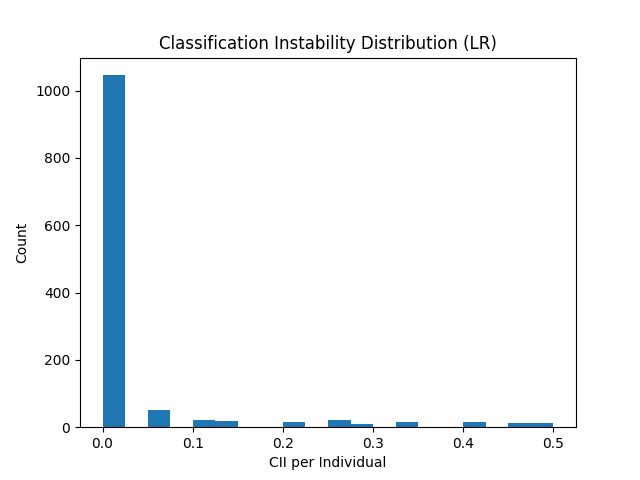
\includegraphics[width=\linewidth]{LR_distribution_plot.png}
\caption{Logistic Regression}
\end{subfigure}
\hfill
\begin{subfigure}{0.32\textwidth}
\centering
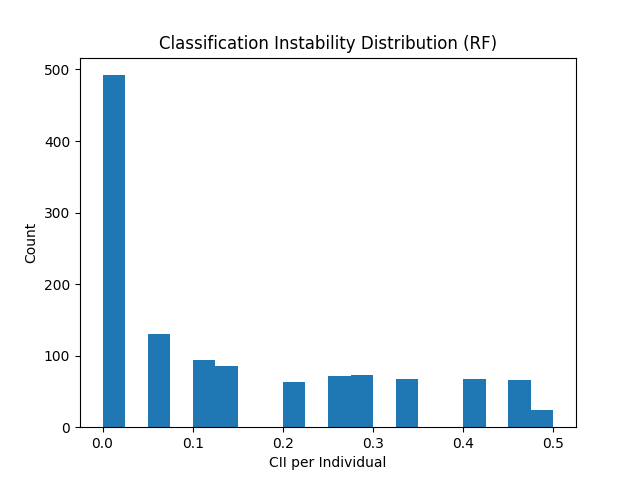
\includegraphics[width=\linewidth]{RF_distribution_plot.png}
\caption{Random Forest}
\end{subfigure}
\hfill
\begin{subfigure}{0.32\textwidth}
\centering
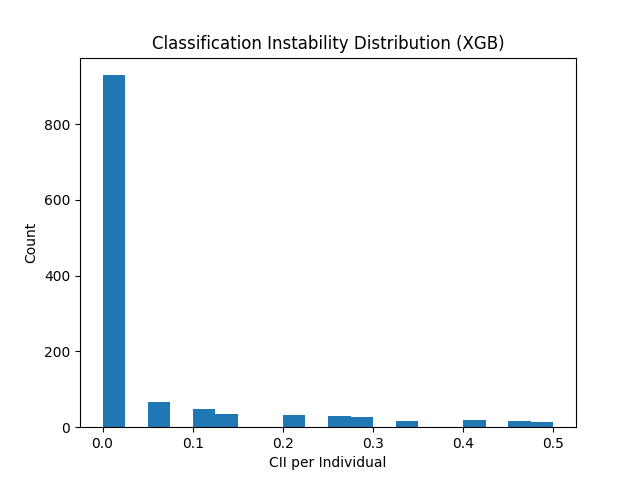
\includegraphics[width=\linewidth]{XGB_distribution_plot.png}
\caption{XGBoost}
\end{subfigure}
\caption{Preliminary CII Distribution Graphs Across Models}
\end{figure}

Figure 2 presents a bard-based summary of CII values across models. This serves as an initial validation that the bootstrap-based sampling procedure produces observable variability in model predictions.

\begin{figure}[h]
\centering
\begin{subfigure}{0.32\textwidth}
\centering
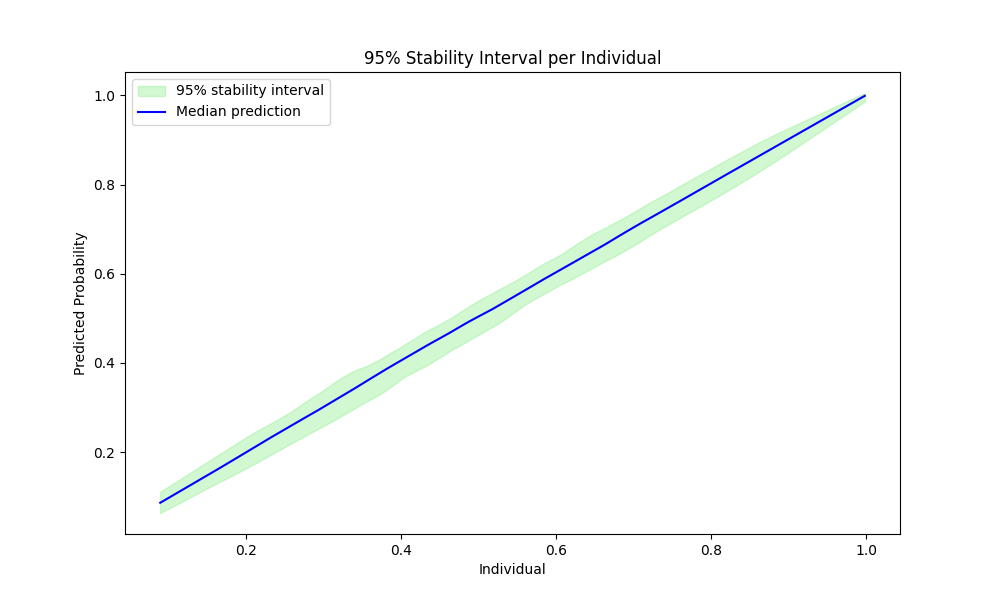
\includegraphics[width=\linewidth]{LR_percentile.png}
\caption{Logistic Regression}
\end{subfigure}
\hfill
\begin{subfigure}{0.32\textwidth}
\centering
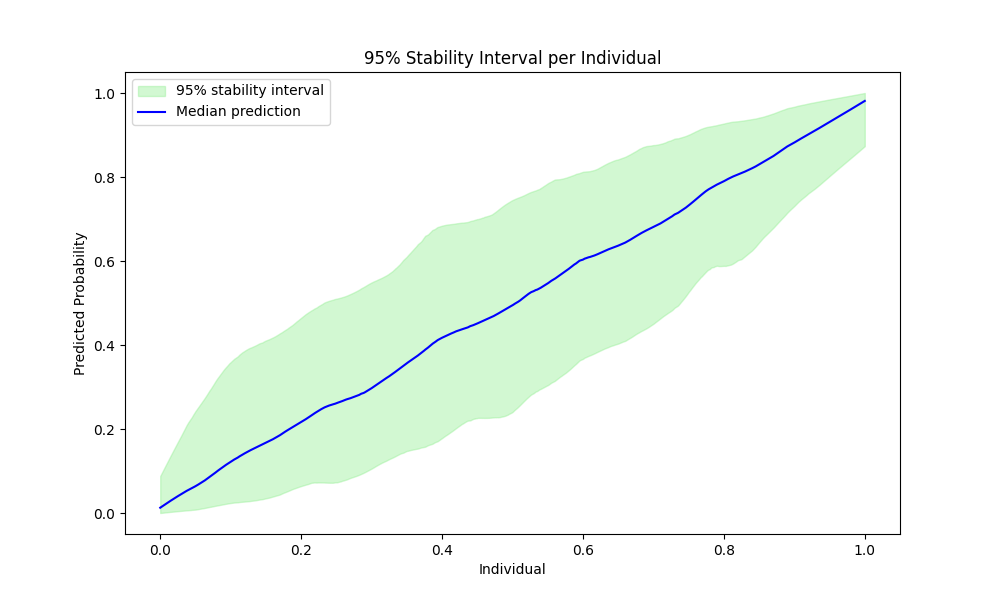
\includegraphics[width=\linewidth]{RF_percentile.png}
\caption{Random Forest}
\end{subfigure}
\hfill
\begin{subfigure}{0.32\textwidth}
\centering
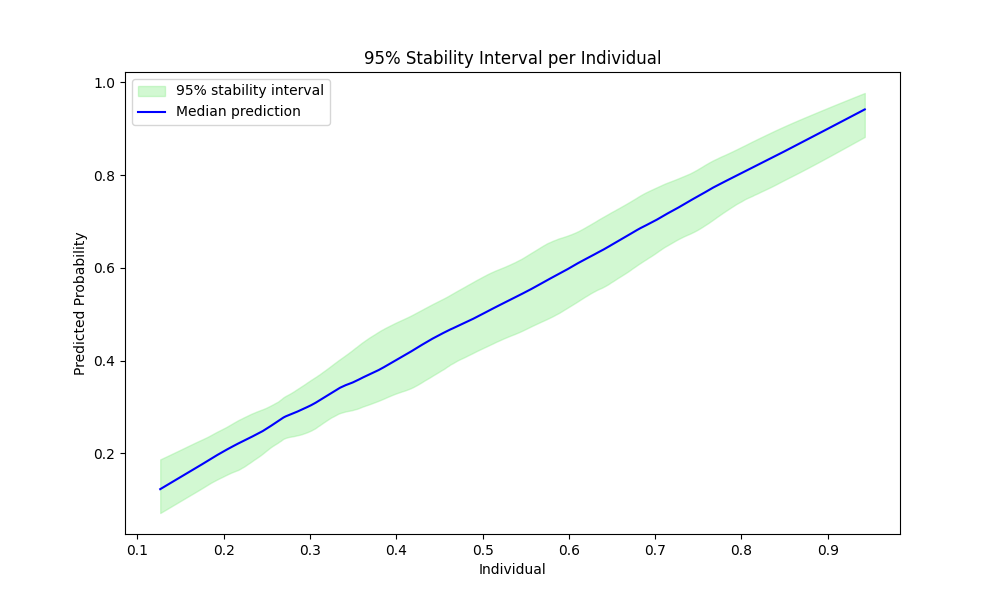
\includegraphics[width=\linewidth]{XGB_percentile.png}
\caption{XGBoost}
\end{subfigure}
\caption{Preliminary 95\% Instability Percentile Across Models}
\end{figure}

Figure 3 summarizes the upper tail of prediction variability using the 95th percentile across runs. This is used as a preliminary indicator of the range of instability observed under repeated sampling. Based on the figure, differences in percentile distributions can be observed across the models.

\newpage
\begin{figure}[h]
\centering
\begin{subfigure}{0.32\textwidth}
\centering
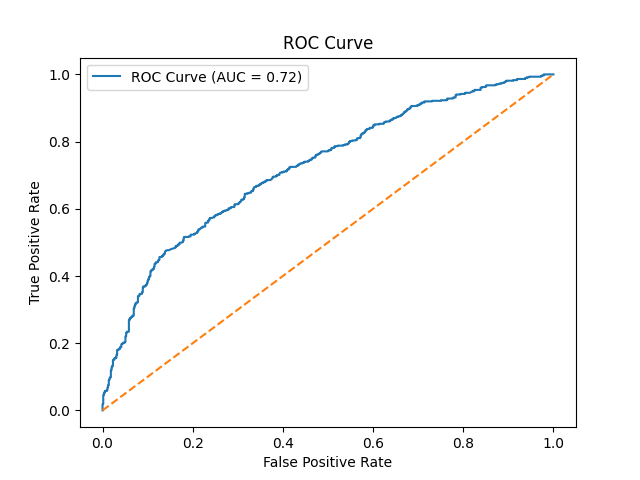
\includegraphics[width=\linewidth]{LR_ROC_20.png}
\caption{Logistic Regression}
\end{subfigure}
\hfill
\begin{subfigure}{0.32\textwidth}
\centering
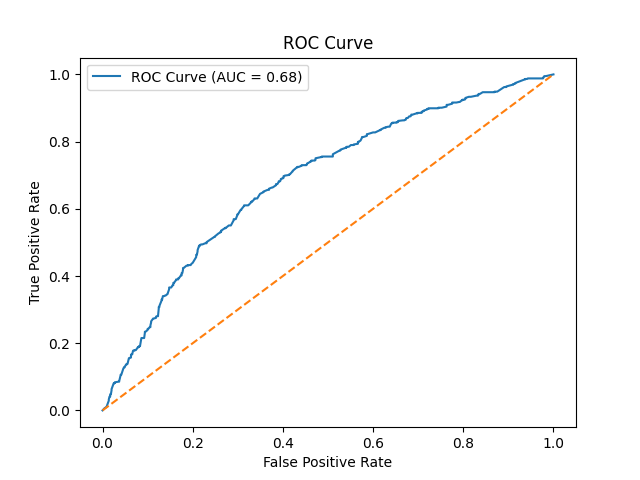
\includegraphics[width=\linewidth]{RF_ROC_20.png}
\caption{Random Forest}
\end{subfigure}
\hfill
\begin{subfigure}{0.32\textwidth}
\centering
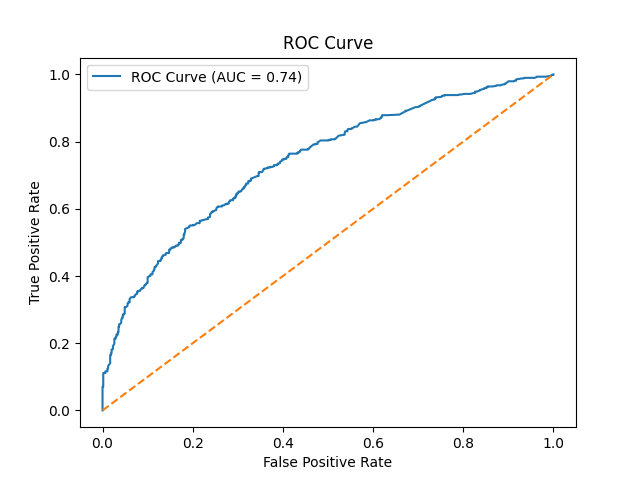
\includegraphics[width=\linewidth]{XGB_ROC_20.png}
\caption{XGBoost}
\end{subfigure}
\caption{Preliminary ROC Curve For Bootstrap Sample 20}
\end{figure}

Figure 4 shows the ROC curves of the evaluated models at bootstrap sample 20 under the current experimental setup. This is included as a preliminary check to verify that the models produce valid probabilistic outputs suitable for downstream evaluation. \\

\newpage
\section{Schedule of Activities}
\subsection{2026}

\begin{longtable}{
 |>{\raggedright\arraybackslash}p{1.1cm}
 |>{\raggedright\arraybackslash}p{2.5cm}
 |>{\raggedright\arraybackslash}p{4cm}
 |*{8}{>{\centering\arraybackslash}p{0.6cm}|}
}
\caption{Schedule of Activities (2026)}\label{tab:schedule}\\
\hline
\textbf{Objective} & \textbf{Target Activities} & \textbf{Target Accomplishments} & \multicolumn{8}{c|}{\textbf{2026 (Months)}} \\
\cline{4-11}
& & & May & Jun & Jul & Aug & Sept & Oct & Nov & Dec \\
\hline
\endfirsthead

\hline
\textbf{Objective} & \textbf{Target Activities} & \textbf{Target Accomplishments} & \multicolumn{8}{c|}{\textbf{2026 (Months)}} \\
\cline{4-11}
& & & May & Jun & Jul & Aug & Sept & Oct & Nov & Dec \\
\hline
\endhead

Obj. 1
& Generate bootstrapped samples from the training dataset and retrain the models to assess dataset instability.
&
(1) Generate bootstrapped samples from the dataset.\newline
(2) Train each model once on the original dataset, then all bootstrapped samples.\newline
(3) Save generated predictions from the fixed test dataset in a csv file.
& \cellcolor{gray!30} & \cellcolor{gray!30} & \cellcolor{gray!30} & \cellcolor{gray!30} & & & & \\
\hline

Obj. 2
& Retrain models on the same dataset with different random seeds to assess stochastic instability.
&
(1) Train each model multiple times using different random seeds, while using the same dataset and model parameters.\newline
(2) Save generated predictions from the fixed test dataset in a csv file.
& \cellcolor{gray!30} & \cellcolor{gray!30} & \cellcolor{gray!30} & \cellcolor{gray!30} & & & & \\
\hline

Obj. 3
& Evaluate each model for each type of instability using metrics for instability, performance, fairness, reliability, and feature contributions using the prediction values obtained. 
&
(1) Measure model instability using instability metrics.\newline
(2) Measure model predictive performance using performance metrics.\newline
(3) Measure model fairness using fairness metrics.\newline
(4) Measure model reliability using a reliability metric.\newline
(5) Use SHAP analysis to identify which features exhibit variability in their contributions across runs. \newline
(6) Save all computed instability, performance, fairness, reliability, and feature contribution results and graphs for analysis.
& & & \cellcolor{gray!30} & \cellcolor{gray!30} & \cellcolor{gray!30} & & & \\
\hline

Obj. 4
& Analyze how results obtained from metrics evaluating each type of instability and model structure influences overall model instability. 
&
(1) Compare results from instability metrics across all models to identify which models exhibit higher dataset and stochastic instability.\newline
(2) Compare results from performance, fairness, and reliability metrics to instability metrics to identify patterns and relationships.\newline
(3) Contextualize model viability using instability metrics with performance, fairness, and reliability metrics.\newline
(4) Analyze the relationship between SHAP-based feature importance and SHAP variability to identify features that are both important and unstable.\newline
(5) Examine patterns in feature contributions across models to determine whether certain features consistently exhibit variability in their contributions across runs.\newline
(6) Synthesize the results to explain overall model instability.
& & & & & \cellcolor{gray!30} & \cellcolor{gray!30} & \cellcolor{gray!30} & \cellcolor{gray!30} \\
\hline

\end{longtable}

\bibliographystyle{unsrt}
\bibliography{references}

\end{document}



\section{Objectives of the Study} 
\subsection{General Objective} Evaluate the instability of classification models used in recidivism risk prediction through dataset and stochastic factors.
\subsection{Specific Objectives}
\begin{enumerate}
 \item Generate bootstrapped samples from the training dataset and retrain the models to assess dataset instability.
 \item Retrain models on the same dataset with different random seeds to assess stochastic instability.
 \item Evaluate each model for each type of instability using metrics for instability, performance, fairness, reliability, and feature contributions using the prediction values obtained. 
 \item Analyze how results obtained from metrics evaluating each type of instability and model structure influences overall model instability. 
\end{enumerate}